\documentclass[12pt, a4paper]{article}

% ── Encodage & langue ──────────────────────────────────────────────────────────
\usepackage[utf8]{inputenc}
\usepackage[T1]{fontenc}
\usepackage[french]{babel}

% ── Mise en page ───────────────────────────────────────────────────────────────
\usepackage[top=2.5cm, bottom=2.5cm, left=2.5cm, right=2.5cm]{geometry}
\usepackage{setspace}
\onehalfspacing

% ── Maths ──────────────────────────────────────────────────────────────────────
\usepackage{amsmath, amssymb, amsthm}

% ── Figures & couleurs ─────────────────────────────────────────────────────────
\usepackage{graphicx}
\usepackage{xcolor}
\usepackage{float}
\usepackage{caption}
\usepackage{subcaption}

% ── Code Python ────────────────────────────────────────────────────────────────
\usepackage{listings}
\definecolor{codebg}{RGB}{248,248,248}
\definecolor{codeframe}{RGB}{200,200,200}
\definecolor{kwcolor}{RGB}{0,112,184}
\definecolor{strcolor}{RGB}{163,21,21}
\definecolor{commentcolor}{RGB}{100,100,100}

\lstdefinestyle{python}{
  language=Python,
  backgroundcolor=\color{codebg},
  frame=single,
  rulecolor=\color{codeframe},
  basicstyle=\ttfamily\small,
  keywordstyle=\color{kwcolor}\bfseries,
  stringstyle=\color{strcolor},
  commentstyle=\color{commentcolor}\itshape,
  showstringspaces=false,
  breaklines=true,
  numbers=left,
  numberstyle=\tiny\color{gray},
  numbersep=8pt,
  tabsize=4,
  captionpos=b,
}

% ── Liens ──────────────────────────────────────────────────────────────────────
\usepackage{hyperref}
\hypersetup{colorlinks=true, linkcolor=black, urlcolor=blue, citecolor=black}

% ── En-tête / pied de page ─────────────────────────────────────────────────────
\usepackage{fancyhdr}
\pagestyle{fancy}
\fancyhf{}
\renewcommand{\headrulewidth}{0.4pt}
\fancyhead[L]{\small Projet S8 — Le restaurant chinois}
\fancyhead[R]{\small Université Paris-Saclay}
\fancyfoot[C]{\thepage}

% ── Environnements maths ───────────────────────────────────────────────────────
\theoremstyle{definition}
\newtheorem{definition}{Définition}[section]
\newtheorem{proposition}{Proposition}[section]
\newtheorem{remarque}{Remarque}[section]
\theoremstyle{plain}
\newtheorem{theoreme}{Théorème}[section]

% ══════════════════════════════════════════════════════════════════════════════
\begin{document}

% ── Page de titre ──────────────────────────────────────────────────────────────
\begin{titlepage}
  \centering
  \vspace*{1cm}

  {\large \textsc{Université Paris-Saclay}}\\[0.3cm]
  {\large L3 — Mathématiques}\\[0.3cm]
  {\normalsize MEU 259 - Projet — Année 2025–2026}

  \vspace{1.5cm}
  \rule{\linewidth}{0.5pt}\\[0.4cm]
  {\huge \bfseries S8 - Le restaurant chinois}\\[0.2cm]
  \rule{\linewidth}{0.5pt}

  \vspace{2cm}

  {\large
  \begin{tabular}{c}
    Owen \textsc{Camilleri} \\[0.5em]
    Maxime \textsc{Hesters} \\[0.5em]
    Aylan \textsc{Khedimallah}
  \end{tabular}
  }

  \vfill

  {\normalsize \ Avril 2026}
\end{titlepage}

% ── Table des matières ─────────────────────────────────────────────────────────
\tableofcontents
\newpage

% ══════════════════════════════════════════════════════════════════════════════
\section{Introduction}

Ce projet a pour objet l'étude d'un processus aléatoire classique, connu sous le nom de
\emph{processus du restaurant chinois}. Ce modèle trouve des applications dans des domaines
aussi variés que la combinatoire des permutations
ou encore la modélisation de processus biologiques.

Le principe est le suivant : des clients arrivent successivement dans un restaurant et
s'assoient selon une règle probabiliste paramétrée par un réel $\theta > 0$. Cette règle
engendre une partition aléatoire de l'ensemble des clients, dont on cherche à comprendre le
comportement asymptotique, à estimer le paramètre $\theta$, et à relier la structure à d'autres
objets mathématiques connus.

Ce rapport est organisé en quatre parties. La première décrit et simule le processus, et en
établit les propriétés asymptotiques. La deuxième traite l'estimation de $\theta$ par deux
méthodes différentes. La troisième exploite le lien avec les permutations uniformes pour
analyser le problème du Secret Santa. Enfin, la quatrième section introduit une généralisation
du processus et son interprétation comme modèle de développement cellulaire.

% ══════════════════════════════════════════════════════════════════════════════
\section{Description, simulation et propriétés}

\subsection{Description du processus}

\begin{definition}[Processus du restaurant chinois]
Soit $\theta > 0$. On considère des clients arrivant successivement dans un restaurant.
Lorsque le $(k+1)$-ème client arrive, $k$ clients sont déjà assis, répartis en tables
d'occupation $(n_1, \ldots, n_p)$ avec $\sum n_i = k$. Alors :
\begin{itemize}
  \item avec probabilité $\dfrac{\theta}{\theta + k}$, il ouvre une nouvelle table (s'assoit seul) ;
  \item avec probabilité $\dfrac{n_i}{\theta + k}$, il s'assoit à la table $i$ existante.
\end{itemize}
\end{definition}

Le paramètre $\theta$ contrôle la tendance à créer de nouvelles tables : plus $\theta$ est
grand, plus le processus est \emph{exploratoire} (beaucoup de petites tables), tandis qu'un
$\theta$ faible favorise le regroupement des clients sur un petit nombre de tables.

\begin{remarque}
  On note $B_n$ le nombre de tables occupées après l'arrivée des $n$ premiers clients.
  La suite $(B_n)$ est croissante et prend ses valeurs dans $\{1, \ldots, n\}$.
\end{remarque}

\subsection{Première simulation : occupation des tables}

Afin de se familiariser avec le modèle, on commence par simuler directement l'occupation
des tables pour différentes valeurs de $\theta$, avec $n = 500$ clients.

\subsubsection*{Implémentation}


L'algorithme repose sur la règle suivante : conditionnellement au fait que le client ne
s'assoit pas seul, il choisit la table $i$ avec probabilité $n_i / k$, proportionnelle à sa
taille. On simule ce choix par une variable uniforme et une recherche séquentielle dans le
tableau des cumuls.

\subsubsection*{Résultats et commentaires}

On trace pour chaque valeur de $\theta \in \{0{,}5,\ 1,\ 1{,}5,\ 10\}$ un diagramme en
barres représentant la taille de chaque table numérotée par ordre d'ouverture.

% ── Placeholder figures ────────────────────────────────────────────────────────
% Remplacer les lignes suivantes par \includegraphics{...} une fois les figures exportées.

\begin{figure}[H]
  \centering
  \begin{subfigure}[b]{0.48\textwidth}
    \centering
    \includegraphics[width=\linewidth]{restaurant_theta_0.5.png}
    \caption{$\theta = 0{,}5$}
  \end{subfigure}
  \hfill
  \begin{subfigure}[b]{0.48\textwidth}
    \centering
    \includegraphics[width=\linewidth]{restaurant_theta_1.png}
    \caption{$\theta = 1$}
  \end{subfigure}

  \vspace{0.5cm}

  \begin{subfigure}[b]{0.48\textwidth}
    \centering
    \includegraphics[width=\linewidth]{restaurant_theta_5.png}
    \caption{$\theta = 5$}
  \end{subfigure}
  \hfill
  \begin{subfigure}[b]{0.48\textwidth}
    \centering
    \includegraphics[width=\linewidth]{restaurant_theta_10.png}
    \caption{$\theta = 10$}
  \end{subfigure}

  \caption{Occupation des tables pour $n = 500$ clients et différentes valeurs de $\theta$.}
  \label{fig:occupation}
\end{figure}

On observe les comportements suivants à partir d'une seule simulation :

\begin{itemize}
  \item Pour $\theta = 0{,}5$, le processus est très concentré : quelques tables accueillent
        la quasi-totalité des clients (ici, on observe seulement 3 tables). La première table ouverte attire naturellement le plus de monde, créant un effet \emph{boule de neige}.

  \item Pour $\theta = 1$, on observe plus de tables qu'avec $\theta = 0{,}5$, et les clients semblent principalement se répartir sur les premières tables.

  \item Pour $\theta = 10$, de nombreuses tables sont ouvertes et restent de petite taille.
        Le processus ressemble davantage à une attribution quasi-uniforme : la probabilité
        d'ouvrir une nouvelle table reste élevée tout au long du processus.
\end{itemize}

\medskip
Ces observations illustrent le rôle fondamental de $\theta$ : il contrôle le compromis
entre \emph{exploration} (nouvelles tables) et \emph{exploitation} (rejoindre une table
existante). Cependant, ces résultats ne sont pas très représentatifs car ils reposent sur une seule simulation, qui peut être très aléatoire.

\medskip
Pour obtenir des conclusions plus robustes, nous allons maintenant simuler le processus \( B_n \) (le nombre de tables occupées après \( n \) clients) sur un grand nombre de répétitions, afin d'étudier son comportement moyen et sa variabilité.

\subsection{Étude asymptotique du nombre de tables}

On rappelle que \( B_n \) désigne le nombre de tables occupées après l'arrivée des \( n \) premiers clients.

\medskip
\noindent
\textbf{Simulations de \( B_n \) :}
Pour étudier le comportement asymptotique de \( B_n \), nous avons simulé ce processus pour différentes valeurs de \(\theta\) et pour \( n \) allant jusqu'à 100 000. Les figures ci-dessous montrent l'évolution de \( B_n \) en fonction de \( n \), ainsi que la moyenne empirique de \( B_n \). Ces simulations permettent de visualiser la croissance de \( B_n \) et sa variabilité.

\begin{figure}[h]
    \centering
    \begin{subfigure}{0.8\textwidth}
        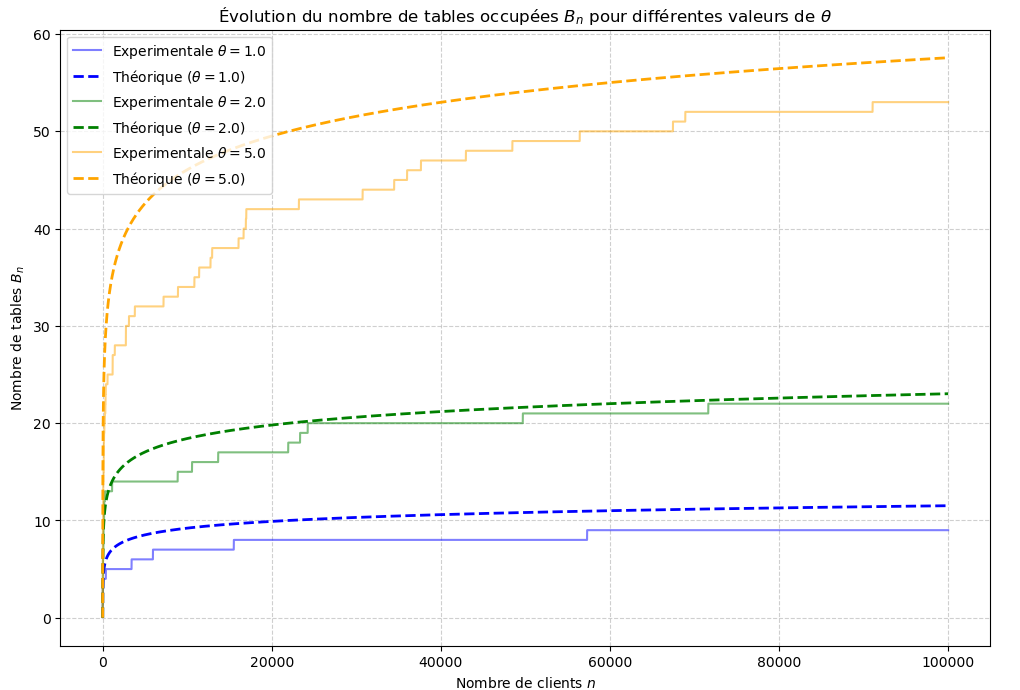
\includegraphics[width=\linewidth]{bn.png}
    \end{subfigure}
    \caption{Évolution de \( B_n \) en fonction de \( n \) pour différentes valeurs de \(\theta\). Chaque courbe représente une valeur de \(\theta\), avec la courbe théorique associée \theta \log n }
\end{figure}

Ces simulations suggèrent que \( B_n \) suit une tendance logarithmique, comme attendu théoriquement. Nous allons maintenant étudier formellement son espérance et sa variance.

\subsubsection*{Décomposition en somme de Bernoulli}

Pour tout $k \geq 1$, on introduit la variable aléatoire
\[
X_k =
\begin{cases}
1 & \text{si le $k$-ième client ouvre une nouvelle table}, \\
0 & \text{sinon}.
\end{cases}
\]

Alors, par construction,
\[
B_n = \sum_{k=1}^n X_k.
\]

De plus, pour tout $k \geq 1$,
\[
\mathbb{P}(X_k = 1) = \frac{\theta}{\theta + k - 1}.
\]

Les variables $(X_k)$ sont indépendantes, car à chaque étape, la décision d'ouvrir une nouvelle table dépend uniquement du nombre de clients déjà présents.

Ainsi, $B_n$ est une somme de variables de Bernoulli indépendantes de paramètres
\[
p_k = \frac{\theta}{\theta + k - 1}.
\]

\subsubsection*{Espérance}

On a vu que
\[
B_n = \sum_{k=1}^n X_k,
\]
où les variables $(X_k)$ sont indépendantes et vérifient
\[
\mathbb{P}(X_k = 1) = \frac{\theta}{\theta + k - 1}.
\]

Ainsi,
\[
\mathbb{E}[B_n] = \sum_{k=1}^n \mathbb{E}[X_k]
= \sum_{k=1}^n \frac{\theta}{\theta + k - 1}.
\]

On pose
\[
S_n = \sum_{k=1}^n \frac{\theta}{\theta + k - 1}.
\]

\paragraph{Comparaison série–intégrale}

Considérons la fonction
\[
f(x) = \frac{\theta}{\theta + x},
\]
qui est décroissante sur $[0,+\infty[$.

Pour tout $k \geq 1$, on a alors
\[
\int_k^{k+1} f(x)\,dx \leq f(k) \leq \int_{k-1}^k f(x)\,dx.
\]

En sommant de $k=1$ à $n$, on obtient
\[
\int_1^{n+1} f(x)\,dx \leq S_n \leq \theta + \int_1^n f(x)\,dx.
\]

\paragraph{Calcul des intégrales}

On calcule
\[
\int_a^b \frac{\theta}{\theta + x}\,dx
= \theta \log(\theta + x)\Big|_a^b
= \theta \log\left(\frac{\theta + b}{\theta + a}\right).
\]

Ainsi,
\[
\int_1^{n+1} f(x)\,dx
= \theta \log\left(\frac{\theta + n + 1}{\theta + 1}\right),
\]
et
\[
\int_1^n f(x)\,dx
= \theta \log\left(\frac{\theta + n}{\theta + 1}\right).
\]

\paragraph{Encadrement}

On en déduit
\[
\theta \log\left(\frac{\theta + n + 1}{\theta + 1}\right)
\leq S_n
\leq
\theta + \theta \log\left(\frac{\theta + n}{\theta + 1}\right).
\]

\paragraph{Comportement asymptotique}

Lorsque $n \to \infty$, on a
\[
\log(\theta + n) \sim \log n
\quad \text{et} \quad
\log(\theta + n + 1) \sim \log n.
\]

Par encadrement, on obtient
\[
S_n \sim \theta \log n.
\]

\paragraph{Conclusion}

Ainsi,
\[
\mathbb{E}[B_n] \sim \theta \log n.
\]

\subsubsection*{Variance}

Comme les variables $(X_k)$ sont indépendantes,
\[
\mathrm{Var}(B_n) = \sum_{k=1}^n \mathrm{Var}(X_k).
\]

Or, pour une variable de Bernoulli,
\[
\mathrm{Var}(X_k) = p_k (1 - p_k).
\]

Donc
\[
\mathrm{Var}(B_n) = \sum_{k=1}^n \frac{\theta}{\theta + k - 1} \left(1 - \frac{\theta}{\theta + k - 1}\right).
\]

Pour $k$ grand,
\[
\mathrm{Var}(X_k) \sim \frac{\theta}{k}.
\]

Ainsi,
\[
\mathrm{Var}(B_n) \sim \theta \sum_{k=1}^n \frac{1}{k}.
\]

Par le même raisonnement que précédemment,
\[
\mathrm{Var}(B_n) \sim \theta \log n.
\]

\subsubsection*{Convergence en probabilité}

On souhaite montrer que
\[
\frac{B_n}{\log n} \xrightarrow[n \to \infty]{\mathbb{P}} \theta.
\]

On applique l'inégalité de Bienaymé–Tchebychev :
\[
\mathbb{P}\left(\left| B_n - \mathbb{E}[B_n] \right| \geq \varepsilon \log n \right)
\leq \frac{\mathrm{Var}(B_n)}{\varepsilon^2 (\log n)^2}.
\]

Or,
\[
\mathrm{Var}(B_n) \sim \theta \log n,
\]

donc
\[
\frac{\mathrm{Var}(B_n)}{(\log n)^2} \sim \frac{\theta}{\log n} \xrightarrow[n \to \infty]{} 0.
\]

Ainsi,
\[
\frac{B_n - \mathbb{E}[B_n]}{\log n} \xrightarrow{\mathbb{P}} 0.
\]

Comme
\[
\frac{\mathbb{E}[B_n]}{\log n} \to \theta,
\]

on obtient finalement
\[
\frac{B_n}{\log n} \xrightarrow{\mathbb{P}} \theta.
\]
\subsubsection*{Convergence presque sûre ? Étude expérimentale}

On peut se demander si la convergence précédente est presque sûre, c’est-à-dire si
\[
\frac{B_n}{\log n} \xrightarrow[n \to \infty]{\text{p.s.}} \theta.
\]

Pour explorer cette question, on utilise la fonction de simulation introduite
précédemment, et on observe l’évolution de la quantité
\[
\frac{B_n}{\log n}
\]
au cours du temps, pour une trajectoire donnée.

\paragraph{Simulation}


On trace la courbe de $B_n / \log n$ en fonction de $n$.

\begin{figure}[H]
  \centering
  \includegraphics[width=0.7\textwidth]{teta.png}
  \caption{Évolution de $B_n / \log n$ en fonction de $n$.}
\end{figure}

\paragraph{Observations}

Les simulations montrent que la quantité $B_n / \log n$ reste proche de $\theta$,
mais continue de fluctuer de manière persistante, même pour des valeurs de $n$
très grandes.

Ces fluctuations ne semblent pas s’atténuer suffisamment pour suggérer une
convergence presque sûre vers $\theta$. La trajectoire oscille autour de la valeur
$\theta$ sans s’en rapprocher de façon stable.

\paragraph{Conclusion}

Ces observations suggèrent qu’il n’y a pas de convergence presque sûre de
$\frac{B_n}{\log n}$ vers $\theta$, mais seulement une convergence en probabilité.

\subsubsection*{Fluctuations asymptotiques et théorème central limite}

On cherche maintenant à décrire plus finement les fluctuations de $B_n$ autour de
son espérance.

On pose
\[
a_n = \theta \log n
\quad \text{et} \quad
b_n = \sqrt{\theta \log n}.
\]

On considère alors la variable centrée et réduite
\[
\frac{B_n - a_n}{b_n}.
\]

Comme $B_n$ est une somme de variables de Bernoulli indépendantes $(X_k)$, on peut
appliquer un théorème central limite pour suites de variables indépendantes.

En effet,
\[
B_n = \sum_{k=1}^n X_k,
\]
avec
\[
\sum_{k=1}^n \mathrm{Var}(X_k) \sim \theta \log n = b_n^2.
\]

On en déduit que
\[
\frac{B_n - \theta \log n}{\sqrt{\theta \log n}}
\xrightarrow[n \to \infty]{\mathcal{L}} \mathcal{N}(0,1).
\]

Ici, on applique une autre version du TCL classique vu en L3, car ici, les variables ne sont pas {iid}, donc les conditions du Théorème Central Limite "classique" ne sont pas vérifiées.

\section{Estimation de $\theta$}

Dans cette partie, on suppose que le paramètre $\theta$ est inconnu, et on cherche à l’estimer à partir de l’observation du processus $(B_n)$.

\subsection{Estimateur asymptotiquement sans biais}

\paragraph{Construction de l’estimateur}

On a montré dans la partie précédente que
\[
\mathbb{E}[B_n] \sim \theta \log n.
\]

Cette relation suggère naturellement de considérer l’estimateur
\[
\hat{\theta}_n = \frac{B_n}{\log n}.
\]

\paragraph{Propriété asymptotique}

On calcule l’espérance de cet estimateur :
\[
\mathbb{E}[\hat{\theta}_n]
= \frac{\mathbb{E}[B_n]}{\log n}.
\]

Or, comme
\[
\mathbb{E}[B_n] \sim \theta \log n,
\]
on obtient
\[
\mathbb{E}[\hat{\theta}_n]
\sim \frac{\theta \log n}{\log n}
= \theta.
\]

\paragraph{Conclusion}

Ainsi, l’estimateur $\hat{\theta}_n$ est asymptotiquement sans biais :
\[
\mathbb{E}[\hat{\theta}_n] \xrightarrow[n \to \infty]{} \theta.
\]

De plus, comme on a montré précédemment que
\[
\frac{B_n}{\log n} \xrightarrow{\mathbb{P}} \theta,
\]
on en déduit que $\hat{\theta}_n$ est également un estimateur consistant.

\subsection{Estimateur du maximum de vraisemblance}

On cherche maintenant à déterminer l’estimateur du maximum de vraisemblance de $\theta$ à partir de l’observation de $(B_1, \dots, B_n)$.

\paragraph{Vraisemblance}

On rappelle que
\[
B_n = \sum_{k=1}^n X_k,
\]
où les variables $(X_k)$ sont indépendantes et
\[
\mathbb{P}(X_k = 1) = \frac{\theta}{\theta + k - 1}.
\]

La vraisemblance s’écrit donc
\[
L(\theta) = \prod_{k=1}^{n} \left( \frac{\theta}{\theta + k - 1} \right)^{X_k}
\left( \frac{k - 1}{\theta + k - 1} \right)^{1 - X_k}.
\]

\paragraph{Log-vraisemblance}

On considère la log-vraisemblance :
\[
\ell(\theta) = \log L(\theta).
\]

On obtient
\[
\ell(\theta)
= \sum_{k=1}^{n} \left[
X_k \log \theta
- \log(\theta + k - 1)
+ (1 - X_k) \log(k - 1)
\right].
\]

Les termes ne dépendant pas de $\theta$ peuvent être ignorés, d’où
\[
\ell(\theta)
= \sum_{k=1}^{n} \left[
X_k \log \theta
- \log(\theta + k - 1)
\right] + \text{constante}.
\]

\paragraph{Dérivation}

On dérive :
\[
\ell'(\theta)
= \sum_{k=1}^{n} \left[
\frac{X_k}{\theta}
- \frac{1}{\theta + k - 1}
\right].
\]

On regroupe :
\[
\ell'(\theta)
= \frac{1}{\theta} \sum_{k=1}^{n} X_k
- \sum_{k=1}^{n} \frac{1}{\theta + k - 1}.
\]

Or,
\[
\sum_{k=1}^{n} X_k = B_n,
\]

donc
\[
\ell'(\theta)
= \frac{B_n}{\theta}
- \sum_{k=1}^{n} \frac{1}{\theta + k - 1}.
\]

\paragraph{Équation du maximum de vraisemblance}

En annulant la dérivée :
\[
\frac{B_n}{\theta}
= \sum_{k=1}^{n} \frac{1}{\theta + k - 1},
\]

soit
\[
B_n = \sum_{k=1}^{n} \frac{\theta}{\theta + k - 1}.
\]


\paragraph{Unicité et de la nature du point critique}

Pour justifier que cette solution est bien un maximum global et qu'elle est unique, considérons les points suivants :

\begin{itemize}
    \item La fonction \( f(\theta) = \sum_{k=0}^{n} \frac{\theta}{\theta + k} \) est \textbf{strictement croissante} en \(\theta\), car chaque terme \(\frac{\theta}{\theta + k}\) est croissant en \(\theta\).
    \item Lorsque \(\theta \to 0^+\), \(f(\theta) \to 0\), et lorsque \(\theta \to +\infty\), \(f(\theta) \to n+1\). Comme \(B_n\) prend ses valeurs dans \(\{1, 2, \dots, n\}\), l'équation \(B_n = f(\theta)\) admet donc \textbf{une unique solution} \(\tilde{\theta}_n\).
    \item La dérivée seconde de la log-vraisemblance est :
    \[
    \ell''(\theta) = -\frac{B_n}{\theta^2} + \sum_{k=1}^{n} \frac{1}{(\theta + k - 1)^2}.
    \]
    Pour \(\theta > 0\), on a \(\ell''(\theta) < 0\) (car \(\frac{B_n}{\theta^2}\) domine), ce qui montre que la log-vraisemblance est \textbf{concave}. Le point critique trouvé est donc bien un \textbf{maximum global}.
\end{itemize}

\paragraph{Conclusion}

L’estimateur du maximum de vraisemblance $\tilde{\theta}_n$ est donc l’unique solution de
\[
B_n = \sum_{k=0}^{n} \frac{\tilde{\theta}_n}{\tilde{\theta}_n + k}.
\]


\paragraph{Comparaison des estimateurs}

On compare deux estimateurs de $\theta$ :
\[
\hat{\theta}_n = \frac{B_n}{\log n}
\quad \text{et} \quad
\tilde{\theta}_n^{\mathrm{}}.
\]

L’estimateur $\hat{\theta}_n^{}$ est simple à calculer mais repose sur un résultat asymptotique, tandis que l’estimateur du maximum de vraisemblance est en général plus précis.

Les simulations montrent que les deux estimateurs convergent vers $\theta$, mais que $\tilde{\theta}_n$ est plus stable pour des tailles finies.

\begin{figure}[h]
    \centering
    \includegraphics[width=0.7\linewidth]{graphe.png}
    \caption{Comparaison des estimateurs de $\theta$ en fonction de $n$.}
\end{figure}

\section{Permutation uniforme : le Secret Santa}

\subsection{Description du problème}

On considère un groupe de $N$ personnes organisant un \emph{Secret Santa}. Le principe est le suivant : chaque personne offre un cadeau à une autre personne, de telle sorte que chacun donne et reçoit exactement un cadeau.

Mathématiquement, cela revient à tirer une permutation $\sigma$ uniformément au hasard dans l’ensemble des permutations de $\{1, \dots, N\}$. La personne $i$ offre alors son cadeau à $\sigma(i)$.

Lors de l’échange, on procède de la manière suivante : la personne $1$ donne son cadeau à $\sigma(1)$, puis la personne $\sigma(1)$ donne son cadeau à $\sigma(\sigma(1))$, et ainsi de suite. On s’intéresse au nombre d’étapes nécessaires pour que la personne $1$ reçoive finalement son propre cadeau. On note ce temps $T$.

\medskip

Ce temps correspond exactement à la taille du cycle de la permutation $\sigma$ contenant l’élément $1$.

\subsection{Lien avec le processus du restaurant chinois pour $\theta = 1$}

On considère maintenant le processus du restaurant chinois dans le cas particulier $\theta = 1$.

Dans ce cas, la règle devient :
\begin{itemize}
  \item le client $k+1$ ouvre une nouvelle table avec probabilité $\dfrac{1}{k+1}$ ;
  \item sinon, il rejoint une table existante avec probabilité proportionnelle à sa taille.
\end{itemize}
\subsection{Lien avec les permutations aléatoires}

Dans le cas particulier où le paramètre $\theta = 1$, le processus du restaurant chinois établit une correspondance avec la structure des cycles d'une permutation aléatoire uniforme de l'ensemble $\{1, \dots, N\}$.

\begin{itemize}
    \item \textbf{Tables et cycles} : Chaque table occupée dans le restaurant correspond à un cycle distinct de la permutation. Autrement dit, le nombre de tables occupées après l'arrivée de $N$ clients est égal au nombre de cycles dans la décomposition de la permutation aléatoire.

    \item \textbf{Taille des tables et longueur des cycles} : La taille $n_i$ de la table $i$ (c'est-à-dire le nombre de clients assis à cette table) est égale à la longueur du cycle $i$ dans la permutation. Par exemple, une table avec 4 clients correspond à un cycle de longueur 4 dans la permutation.

    \item \textbf{Client 1 et cycle contenant 1} : La taille de la table à laquelle le premier client (client 1) est assis a exactement la même loi que la longueur du cycle contenant l'élément 1 dans la permutation aléatoire. Cela signifie que si l'on note $U_N$ la taille de la table contenant le client 1 après l'arrivée de $N$ clients, alors $U_N$ suit la même distribution que la longueur du cycle contenant 1 dans une permutation aléatoire de $\{1, \dots, N\}$.
\end{itemize}



\textbf{Conséquence directe} :
La variable aléatoire $T$, qui représente le temps nécessaire pour que le client 1 reçoive son cadeau dans le cadre du Secret Santa, est donc distribuée de la même manière que $U_N$ :
\[
T \overset{(d)}{=} U_N.
\]

\subsection{Loi uniforme de $T$ et $U_N$}

On montre maintenant que la variable aléatoire \(T\), représentant la longueur du cycle contenant l'élément 1 dans une permutation aléatoire uniforme de \(\{1, 2, \dots, N\}\), suit une loi uniforme sur \(\{1, 2, \dots, N\}\).
\begin{itemize}
    \item Le nombre total de permutations de \(N\) éléments est \(N!\).
    \item Pour tout \(k \in \{1, 2, \dots, N\}\), le nombre de permutations où le cycle contenant 1 a une longueur exactement \(k\) est \((N-1)!\).
    \begin{itemize}
        \item On choisit \(k-1\) éléments parmi les \(N-1\) restants pour former le cycle avec 1 : \(\binom{N-1}{k-1}\) choix.
        \item On arrange ces \(k\) éléments en un cycle : \((k-1)!\) façons.
        \item On permute les \(N-k\) éléments restants : \((N-k)!\) façons.
        \item Le produit est \(\binom{N-1}{k-1} \times (k-1)! \times (N-k)! = (N-1)!\).
    \end{itemize}
    \item La probabilité que \(T = k\) est donc :
    \[
    \mathbb{P}(T = k) = \frac{(N-1)!}{N!} = \frac{1}{N}.
    \]
\end{itemize}

\paragraph{Conclusion}
La variable \(T\) suit une loi uniforme sur \(\{1, 2, \dots, N\}\). Comme \(T \overset{(d)}{=} U_N\), la taille de la table contenant le client 1 dans le processus du restaurant chinois pour \(\theta = 1\) suit également une loi uniforme sur \(\{1, 2, \dots, N\}\).

\begin{figure}[h]
    \centering
    \includegraphics[width=0.8\linewidth]{mon_graphe.png}
    \caption{Correspondance entre les tables du restaurant chinois et les cycles d’une permutation.}
\end{figure}

\subsection{Lien avec les urnes de Pólya}

Considérons une urne de Pólya initiale contenant une boule rouge et une boule bleue. À chaque étape $n+1$, on tire une boule au hasard et on la remplace en ajoutant une boule de la même couleur. Soit $R_n$ le nombre de boules rouges à l'étape $n$. La dynamique de l'urne est la suivante : 

\begin{itemize}
    \item Avec probabilité $\frac{R_n}{n}$, on tire une boule rouge, et on ajoute une boule rouge supplémentaire. Ainsi, $R_{n+1} = R_n + 1$.
    \item Avec probabilité $\frac{B_n}{n} = \frac{n - R_n}{n}$, on tire une boule bleue, et on ajoute une boule bleue supplémentaire. Ainsi, $R_{n+1} = R_n$.
\end{itemize}

\subsubsection{Analogie avec le restaurant chinois}

Dans le processus du restaurant chinois avec $\theta = 1$, notons $U_n$ le nombre de personnes à la table 1 après l'arrivée de $n$ clients. La dynamique de $U_n$ est la suivante :

\begin{itemize}
    \item Le $(n+1)$-ème client s'assoit à la table 1 avec probabilité $\frac{U_n}{n}$ (car la probabilité de s'asseoir à une table est proportionnelle au nombre de clients déjà assis à cette table). Dans ce cas, $U_{n+1} = U_n + 1$.
    \item Sinon, le $(n+1)$-ème client s'assoit à une autre table ou à une nouvelle table, et $U_{n+1} = U_n$.
\end{itemize}

\subsubsection{Comparaison des dynamiques}

Les deux processus partagent la même dynamique probabiliste :
\[
\begin{cases}
P(R_{n+1} = R_n + 1) = \frac{R_n}{n}, \\
P(R_{n+1} = R_n) = \frac{n - R_n}{n},
\end{cases}
\]
et
\[
\begin{cases}
P(U_{n+1} = U_n + 1) = \frac{U_n}{n}, \\
P(U_{n+1} = U_n) = \frac{n - U_n}{n}.
\end{cases}
\]

De plus, les deux processus partagent la même \textbf{condition initiale} :
\[
U_1 = R_1 = 1.
\]

Ainsi, les processus $(R_n)_{n \geq 1}$ et $(U_n)_{n \geq 1}$ sont identiques en loi. Cela signifie que le nombre de personnes à la table 1 dans le restaurant chinois suit la même distribution que le nombre de boules rouges dans l'urne de Pólya.

\subsection{Convergence presque sûre de \( U_N / N \)}

On utilise le modèle de l'urne de Pólya pour étudier la convergence de \( U_N / N \).

\paragraph{Lien avec l'urne de Pólya}
Le processus du restaurant chinois pour \(\theta = 1\) est équivalent à une urne de Pólya contenant initialement une boule rouge (la table du client 1) et une boule bleue (les autres tables). À chaque étape :
\begin{itemize}
    \item Si on tire une boule rouge, on la remplace par deux boules rouges.
    \item Si on tire une boule bleue, on la remplace par une boule rouge et une boule bleue.
\end{itemize}
Ainsi, si à l'étape \(N\) il y a \(a\) boules rouges et \(b\) boules bleues, alors à l'étape \(N+1\) :
\begin{itemize}
    \item Avec probabilité \(\frac{a}{a+b}\), on a \(a+1\) boules rouges.
    \item Avec probabilité \(\frac{b}{a+b}\), on a \(a\) boules rouges.
\end{itemize}
L'espérance du nombre de boules rouges à l'étape \(N+1\) sachant l'étape \(N\) est donc :
\[
\mathbb{E}[a_{N+1} | a_N = a] = a.
\]

\paragraph{Utilisation des martingales}
Une martingale est un processus aléatoire \((M_N)\) tel que \(\mathbb{E}[M_{N+1} | M_N] = M_N\). Ici, le nombre de boules rouges \((a_N)\) est une martingale car :
\[
\mathbb{E}[a_{N+1} | a_N] = a_N.
\]

\paragraph{Loi limite}
Dans le cas de l'urne de Pólya avec une boule rouge et une boule bleue initialement, la loi limite de \( M_\infty \) est la loi uniforme sur \([0,1]\). Ainsi :
\[
\frac{U_N}{N} \xrightarrow[N \to \infty]{p.s.} M_\infty,
\]
où \( M_\infty \) suit une loi uniforme sur \([0,1]\).

\paragraph{Interprétation}
Cela signifie que, dans le cadre du restaurant chinois pour \(\theta = 1\), la proportion de clients à la table du client 1 converge presque sûrement vers une variable aléatoire uniformément distribuée entre 0 et 1.

\subsection{Équivalent de \(\mathbb{E}[T]\) lorsque \(N \to \infty\)}

On cherche un équivalent de l'espérance \(\mathbb{E}[T]\) lorsque \(N \to \infty\), où \(T\) est la longueur du cycle contenant l'élément 1 dans une permutation aléatoire uniforme de \(\{1, 2, \dots, N\}\).

\paragraph{Loi de \(T\)}
On a montré que \(T\) suit une loi uniforme sur \(\{1, 2, \dots, N\}\). Ainsi, pour tout \(k \in \{1, 2, \dots, N\}\), on a :
\[
\mathbb{P}(T = k) = \frac{1}{N}.
\]

\paragraph{Calcul de \(\mathbb{E}[T]\)}
L'espérance de \(T\) est donnée par :
\[
\mathbb{E}[T] = \sum_{k=1}^N k \cdot \mathbb{P}(T = k) = \frac{1}{N} \sum_{k=1}^N k = \frac{1}{N} \cdot \frac{N(N+1)}{2} = \frac{N+1}{2}.
\]

\paragraph{Équivalent asymptotique}
Pour \(N\) grand, on obtient l'équivalent suivant :
\[
\mathbb{E}[T] = \frac{N+1}{2} \sim \frac{N}{2}.
\]

\paragraph{Interprétation}
Cela signifie que, en moyenne, la longueur du cycle contenant l'élément 1 dans une permutation aléatoire uniforme de taille \(N\) est de l'ordre de \(N/2\) lorsque \(N\) devient grand.

\subsection{Comparaison avec \(N/\mathbb{E}[B_N]\) et paradoxe apparent}

On compare maintenant l'équivalent de \(\mathbb{E}[T]\) avec une estimation de la taille d'une table typique dans le restaurant chinois.

\paragraph{Rappel des résultats}
\begin{itemize}
    \item L'espérance de \(T\) est \(\mathbb{E}[T] \sim \frac{N}{2}\).
    \item Le nombre moyen de tables est \(\mathbb{E}[B_N] \sim \log N\), donc une estimation de la taille d'une table typique serait \(\frac{N}{\mathbb{E}[B_N]} \sim \frac{N}{\log N}\).
\end{itemize}

\paragraph{Comparaison}
Il y a une différence marquée entre ces deux quantités :
\begin{itemize}
    \item \(\mathbb{E}[T] \sim \frac{N}{2}\) est d'ordre \(N\).
    \item \(\frac{N}{\log N}\) est d'ordre \(N/\log N\), beaucoup plus petit que \(N\) pour \(N\) grand.
\end{itemize}

\paragraph{Explication du "paradoxe"} :

Cette différence n'est pas un vrai paradoxe, mais reflète la \textbf{distribution très déséquilibrée des tailles de tables} dans le processus du restaurant chinois :
\begin{itemize}
    \item La taille moyenne d'une table (\(N/\log N\)) est petite car il y a beaucoup de petites tables.
    \item Cependant, la taille moyenne du cycle contenant 1 (\(N/2\)) est grande car ce cycle a une chance significative d'être l'un des rares grands cycles dans la permutation.
\end{itemize}

\paragraph{Interprétation}
Dans le restaurant chinois, la plupart des tables sont petites, mais il y a quelques tables très grandes. Le cycle contenant 1 a une probabilité non négligeable d'être l'une de ces grandes tables, ce qui explique pourquoi sa taille moyenne est bien plus grande que la taille moyenne d'une table "typique".

\subsection{Secret Santa avec dérangements}

Pour éviter qu'une personne tire son propre nom dans le Secret Santa, il est plus judicieux de choisir \(\sigma\) parmi les permutations sans point fixe, appelées \textbf{dérangements}.

\paragraph{Définition}
Un dérangement est une permutation \(\sigma\) de \(\{1, 2, \dots, N\}\) telle que \(\sigma(i) \neq i\) pour tout \(i\). Le nombre de dérangements de \(N\) éléments est donné par :
\[
!N = N! \sum_{k=0}^N \frac{(-1)^k}{k!}.
\]

\paragraph{Simulation}
On simule le processus du Secret Santa pour des permutations uniformes et pour des dérangements, et on compare la longueur du cycle contenant 1 (notée \(T\)) dans les deux cas.

\begin{figure}[h]
    \centering
    \includegraphics[width=1\linewidth]{derangement2.png}
    \caption{Comparaison de la taille du cycle contenant 1 avec permutations et dérangements, avec 50 clients, 10 000 simulations}
\end{figure}


\paragraph{Interprétation}

Bien que les dérangements excluent les points fixes, la longueur moyenne du cycle contenant 1 reste similaire à celle des permutations uniformes. Cela montre que la contrainte des dérangements n'affecte pas significativement la taille moyenne des cycles, mais peut modifier légèrement leur distribution.

Pour les dérangements, bien que la contrainte de ne pas avoir de point fixe modifie légèrement la distribution des longueurs de cycle, l'espérance de \( T \) reste asymptotiquement proche de celle des permutations uniformes. Ainsi, pour \( N \) grand, on a :
\[
\mathbb{E}[T] \approx \frac{N}{2}.
\]

\paragraph{Justification}
La raison en est que, pour \( N \) grand, la probabilité qu'un élément particulier (comme l'élément 1) soit dans un cycle de longueur donnée est presque la même dans un dérangement que dans une permutation uniforme. La contrainte de ne pas avoir de points fixes affecte principalement les petits cycles, mais a peu d'impact sur les cycles de grande taille.


Choisir \(\sigma\) parmi les dérangements est une approche plus maline pour le Secret Santa, car elle évite les auto-attributions. Cependant, cela ne change pas radicalement le comportement asymptotique de la longueur des cycles.

\section{Une généralisation et un processus biologique}

\subsection{Vérification du modèle généralisé}

Soit un instant où $k$ clients sont répartis sur $p$ tables d'occupations respectives $(n_{1},...,n_{p})$. Les probabilités d'affectation du $(k+1)$-ème client sont données par :
\begin{itemize}
    \item $P(\text{table } i) = \frac{n_{i}-\alpha}{k+\theta}$ pour $i \in \{1, \dots, p\}$.
    \item $P(\text{nouvelle table}) = \frac{\theta+p\alpha}{k+\theta}$.
\end{itemize}

\textbf{Vérification de la loi de probabilité :}
La somme de ces probabilités doit valoir 1. 
$$ \sum_{i=1}^{p} \left( \frac{n_{i}-\alpha}{k+\theta} \right) + \frac{\theta+p\alpha}{k+\theta} = \frac{\sum_{i=1}^{p} n_{i} - p\alpha + \theta + p\alpha}{k+\theta}. $$
Puisque la somme des effectifs des tables est le nombre total de clients $\sum_{i=1}^{p} n_{i} = k$, on obtient bien :
$$ \frac{k - p\alpha + \theta + p\alpha}{k+\theta} = \frac{k+\theta}{k+\theta} = 1. $$

\textbf{Généralisation du restaurant de base :}
Si l'on fixe $\alpha=0$, on retrouve $P(\text{table } i) = \frac{n_{i}}{k+\theta}$ et $P(\text{nouvelle table}) = \frac{\theta}{k+\theta}$, ce qui correspond rigoureusement au modèle initial du restaurant chinois.

\begin{figure}[H]
  \centering
  \begin{subfigure}[b]{0.57\textwidth}
    \centering
    \includegraphics[width=\linewidth]{ho.png}
  \end{subfigure}
\end{figure}

\subsection{Horloges aléatoires et lien formel avec le processus biologique}

Analysons le modèle biologique en temps continu décrit par des horloges exponentielles. Considérons l'état du système à l'instant où l'organisme contient exactement $k$ cellules, réparties en $p$ types (organes) de tailles $(n_{1},...,n_{p})$. 

Par construction du modèle, chaque organe de taille $n_{i}$ est constitué d'exactement \textbf{1 cellule-souche} (la fondatrice) et de \textbf{$n_{i}-1$ cellules-clones}.

Calculons l'intensité (le taux) d'occurrence pour chaque événement de naissance possible :
\begin{enumerate}
    \item \textbf{Création d'une nouvelle cellule-clone dans l'organe $i$ (agrandissement de la table $i$) :}
    \begin{itemize}
        \item La cellule-souche de type $i$ produit un clone avec une intensité $1-\alpha$.
        \item Chacune des $(n_{i}-1)$ cellules-clones de type $i$ produit un clone avec une intensité $1$.
    \end{itemize}
    L'intensité totale de création d'un clone pour l'organe $i$ est donc :
    $$ \lambda_{\text{clone}, i} = (1-\alpha) + (n_{i}-1)\times 1 = n_{i} - \alpha. $$

    \item \textbf{Création d'une nouvelle cellule-souche d'un type inédit (création d'une nouvelle table) :}
    \begin{itemize}
        \item L'horloge globale produit de nouvelles souches avec une intensité $\theta$.
        \item Chacune des $p$ cellules-souches existantes produit une nouvelle souche d'un type nouveau avec une intensité $\alpha$.
    \end{itemize}
    L'intensité totale de création d'un nouvel organe est :
    $$ \lambda_{\text{nouvel organe}} = \theta + p\alpha. $$
\end{enumerate}

\textbf{Probabilités de transition de la chaîne de Markov incluse :}
L'intensité totale $\Lambda$ de création d'une cellule (quelle qu'elle soit) est la somme de toutes les intensités :
$$ \Lambda = \lambda_{\text{nouvel organe}} + \sum_{i=1}^{p} \lambda_{\text{clone}, i} = (\theta + p\alpha) + \sum_{i=1}^{p} (n_{i} - \alpha) = \theta + p\alpha + \left(\sum_{i=1}^{p} n_{i}\right) - p\alpha. $$
Puisque $\sum n_{i} = k$, on a $\Lambda = k + \theta$.

La probabilité que le prochain événement (la $(k+1)$-ème cellule) soit un ajout à l'organe $i$ est le rapport de l'intensité de cet événement sur l'intensité totale :
$$ P(\text{ajout à l'organe } i) = \frac{\lambda_{\text{clone}, i}}{\Lambda} = \frac{n_{i}-\alpha}{k+\theta}. $$
La probabilité que le prochain événement soit la création d'un nouvel organe est :
$$ P(\text{nouvel organe}) = \frac{\lambda_{\text{nouvel organe}}}{\Lambda} = \frac{\theta+p\alpha}{k+\theta}. $$

\textbf{Conclusion :} La suite discrète des naissances de cellules et de leurs affectations aux différents organes suit rigoureusement la loi du processus du restaurant chinois généralisé de paramètres $(\alpha, \theta)$.

\subsection{Estimations asymptotiques du développement de l'organisme}

L'introduction du paramètre $\alpha > 0$ modifie fondamentalement la dynamique du système asymptotique par rapport au modèle classique ($\alpha=0$).

\textbf{Évolution du nombre d'organes (le nombre de tables $B_{k}$) :}
Déterminons l'espérance conditionnelle du nombre d'organes à l'étape $k+1$ :
$$ \mathbb{E}[B_{k+1} | \mathcal{F}_{k}] = B_{k} + P(\text{nouvelle table à l'étape } k+1) = B_{k} + \frac{\theta+B_{k}\alpha}{k+\theta}. $$
En prenant l'espérance totale :
$$ \mathbb{E}[B_{k+1}] = \mathbb{E}[B_{k}] \left( 1 + \frac{\alpha}{k+\theta} \right) + \frac{\theta}{k+\theta}. $$
Contrairement à la récurrence $\mathbb{E}[B_{k+1}] = \mathbb{E}[B_{k}] + \frac{\theta}{k+\theta}$ du cas $\alpha=0$ qui donne une croissance logarithmique $\sim \theta \ln k$, le terme multiplicatif dominant ici est $\left(1 + \frac{\alpha}{k}\right)$.
Par développement asymptotique (similaire à l'étude de la fonction Gamma), on montre que le nombre d'organes croît selon une \textbf{loi de puissance} :
$$ \mathbb{E}[B_{k}] \sim C \cdot k^{\alpha} \quad (k \rightarrow \infty), $$
où $C$ dépend de $\theta$ et $\alpha$. Presque sûrement, $\frac{B_{k}}{k^{\alpha}}$ converge vers une variable aléatoire suivant une loi de Mittag-Leffler. Le paramètre $\alpha$ contrôle ainsi l'explosion de la diversité structurelle de l'organisme.

\textbf{Évolution de la taille des organes :}
Puisqu'il y a au total $k$ cellules réparties en un ordre de grandeur de $k^{\alpha}$ organes, la taille moyenne d'un organe (d'une table) est asymptotiquement :
$$ \text{Taille moyenne} \approx \frac{k}{B_{k}} \sim k^{1-\alpha}. $$
Le processus de Pitman-Yor est bien connu pour générer des partitions exhibant un comportement structurel de type \textit{loi de puissance} (power-law). Cela traduit biologiquement le fait que quelques organes très anciens (créés dans les premières étapes) vont drainer la majorité des cellules (macroscopiques), tandis qu'une myriade de micro-organes récents ne comporteront que très peu de cellules.

\section*{Conclusion}
\addcontentsline{toc}{section}{Conclusion}

Dans ce projet, nous avons étudié en détail le processus du restaurant chinois, un modèle probabiliste fondamental permettant de générer des partitions aléatoires d’un ensemble. Nous avons mis en évidence l’influence du paramètre $\theta > 0$ , à travers des simulations et l’étude asymptotique du nombre de tables $B_n$.

Nous avons ensuite proposé deux estimateurs de $\theta$ : l’un asymptotiquement sans biais, l’autre du maximum de vraisemblance et comparé leurs performances. La mise en relation avec les permutations uniformes (problème du \textit{Secret Santa}) a permis d’interpréter le cas $\theta = 1$ comme un cycle aléatoire uniforme, et de lever un apparent paradoxe sur la taille moyenne des tables.

Enfin, la généralisation du processus (modèle de Pitman–Yor) introduit un second paramètre $\alpha$, dont nous avons montré qu’il modifie radicalement le comportement asymptotique : le nombre de tables croît alors comme une puissance $k^\alpha$, ce qui trouve une interprétation naturelle en biologie du développement.

Ce projet illustre ainsi la richesse des processus de renforcement, leur lien avec la combinatoire, la statistique et la modélisation biologique. Il peut ouvrir la voie à des prolongements tels que l’estimation conjointe de $(\theta, \alpha)$.


$$$$

Convergence presque-sûr ?
Pour n = $10^{6}$
on observe toujours des oscillations “aléatoires” autour de \theta

\end{document}






